\documentclass[UTF8,a4paper,11pt,fontset=fandol]{ctexart}
\usepackage{geometry}
\geometry{margin=2.2cm}
\usepackage{amsmath,amssymb,longtable,booktabs,array,hyperref,xcolor,enumitem,graphicx,float}
\hypersetup{colorlinks=true,linkcolor=blue,urlcolor=blue}
\setlist[itemize]{leftmargin=1.3em,itemsep=0.2em}
\definecolor{notegray}{RGB}{246,248,251}
\title{P03. Cooperation Method of Connected and Automated Vehicles at Unsignalized Intersections: Lane Changing and Arrival Scheduling\\中英双语博士精读笔记}
\author{Chaoyi Chen; Mengchi Cai; Jiawei Wang; Kai Li; Qing Xu; Jianqiang Wang; Keqiang Li}
\date{2021 · arXiv preprint}
\begin{document}
\maketitle

\noindent\textbf{Theme / 主题：} Lane changing + arrival scheduling\\
\textbf{Method family / 方法族：} Lane assignment + arrival scheduling / 车道分配与到达调度\\
\textbf{PDF pages / 页数：} 14 \quad
\textbf{Relevance / 相关度：} 82/100\\
\textbf{Source / 来源：} \url{https://arxiv.org/abs/2109.14175}

\section{论文全景速览与核心贡献 / High-Level Overview \& Core Contributions}
\subsection{研究背景与痛点 / Background \& Pain Points}
这篇论文位于“Lane changing + arrival scheduling”方向。对你的 JSSP-based Intersection Management 课题，它回答的是高层调度、低层轨迹平滑、安全过滤或真实验证中的一个关键子问题：如何让车辆在路口少停、少冲突、少能耗，同时保持在线可执行。

The paper belongs to the theme of Lane changing + arrival scheduling. For a JSSP-based intersection-management thesis, it illuminates one of the key layers: scheduling, smoothing, safety filtering, or real-world validation.

\textbf{Pain point / 痛点：} arXiv note reports text overlap with the authors' earlier graph-based paper; use mainly for lane-changing extension context.

\subsection{核心科学问题 / Core Scientific Question}
当车辆可以变道或选择目标车道时，如何联合决定路径/车道与无冲突到达时间？

How should target-lane assignment and conflict-free arrival scheduling be coupled when vehicles may change lanes before the intersection?

\subsection{科学贡献 / Scientific Contributions}
\begin{itemize}
\item 方法贡献 (method contribution)：Two-stage framework decoupling lateral lane assignment/path planning from graph-based arrival scheduling with minimum clique cover.
\item 安全/避碰贡献 (safety contribution)：Conflict-free arrival scheduling and formation-control assumptions prevent incompatible movements.
\item 平滑/停止避免贡献 (smoothing contribution)：Improves traffic efficiency by choosing target lanes and arrival schedules that avoid unnecessary queuing.
\item 创新力度评判 (reviewer judgement)：中等：在 P02 图排序基础上加入横向决策，扩展性有价值，但理论新颖性主要来自组合而非新算法。
\end{itemize}


\subsection{核心概念对照 / Core Concepts}
\begin{longtable}{p{0.24\linewidth}p{0.28\linewidth}p{0.40\linewidth}}
\toprule
中文概念 & English Concept & Role / 学术作用\\
\midrule
自动交叉口管理 & Autonomous Intersection Management & 把信号控制替换为车辆级调度与控制。 \\
轨迹平滑 & Trajectory Smoothing & 减少急加减速、停车和能耗峰值。 \\
安全约束 & Safety Constraints & 把碰撞风险写成距离、时间间隔或屏障函数。 \\
Lane assignment + arrival scheduling & 车道分配与到达调度 & 该论文的核心方法族。 \\
\bottomrule
\end{longtable}

\section{教材式学习路径与关键截图 / Textbook-Style Study Path \& PDF Snapshots}
\subsection{学习路径 / Study Path}
\begin{itemize}
\item 第一遍先读首页截图、摘要与引言，确认研究问题和场景假设。
\item 第二遍沿着技术路线图复现模型变量、约束和求解器输入输出。
\item 第三遍逐节阅读 section deep reading，对照 PDF 截图检查公式、图表和实验。
\item 第四遍只站在审稿人视角重读实验，判断 baseline、公平性、消融和鲁棒性。
\item 最后把博士 checklist 写成自己的复现实验或论文拓展计划。
\end{itemize}


\subsection{博士阅读 Checklist / Doctoral Reading Checklist}
\begin{itemize}
\item 能否独立重写核心公式：联合车道分配与到达时间优化 / Joint lane assignment and arrival scheduling，并解释每个符号的物理意义？
\item 能否画出输入-模型-算法-控制-验证的数据流图？
\item 能否指出至少两个强假设，并说明它们在真实交通中何时失效？
\item 能否复述实验基准是否公平，指标是否覆盖效率、安全、能耗和计算时间？
\item 能否提出一个与自己 JSSP/RL/smoother 课题直接相连的拓展实验？
\end{itemize}


\subsection{关键截图讲解 / PDF Snapshot Explanation}
Screenshots are selected anchors from the local PDFs for study and parallel reading. They do not replace the original paper.

\begin{figure}[H]
\centering

\includegraphics[width=0.92\linewidth]{../../assets/P03_chen2021lanechanging/01_title_and_abstract_p1.jpg}
\caption{首页与摘要 / Title and abstract page (p.1, full\_page). 这张截图用于把笔记中的抽象概念拉回原论文页面，便于你平行阅读原文、公式、图表和实验设置。 与当前课题的连接：Useful for discussing route-template/lane-choice extensions beyond the current fixed-route JSSP formulation.}
\end{figure}

\begin{figure}[H]
\centering
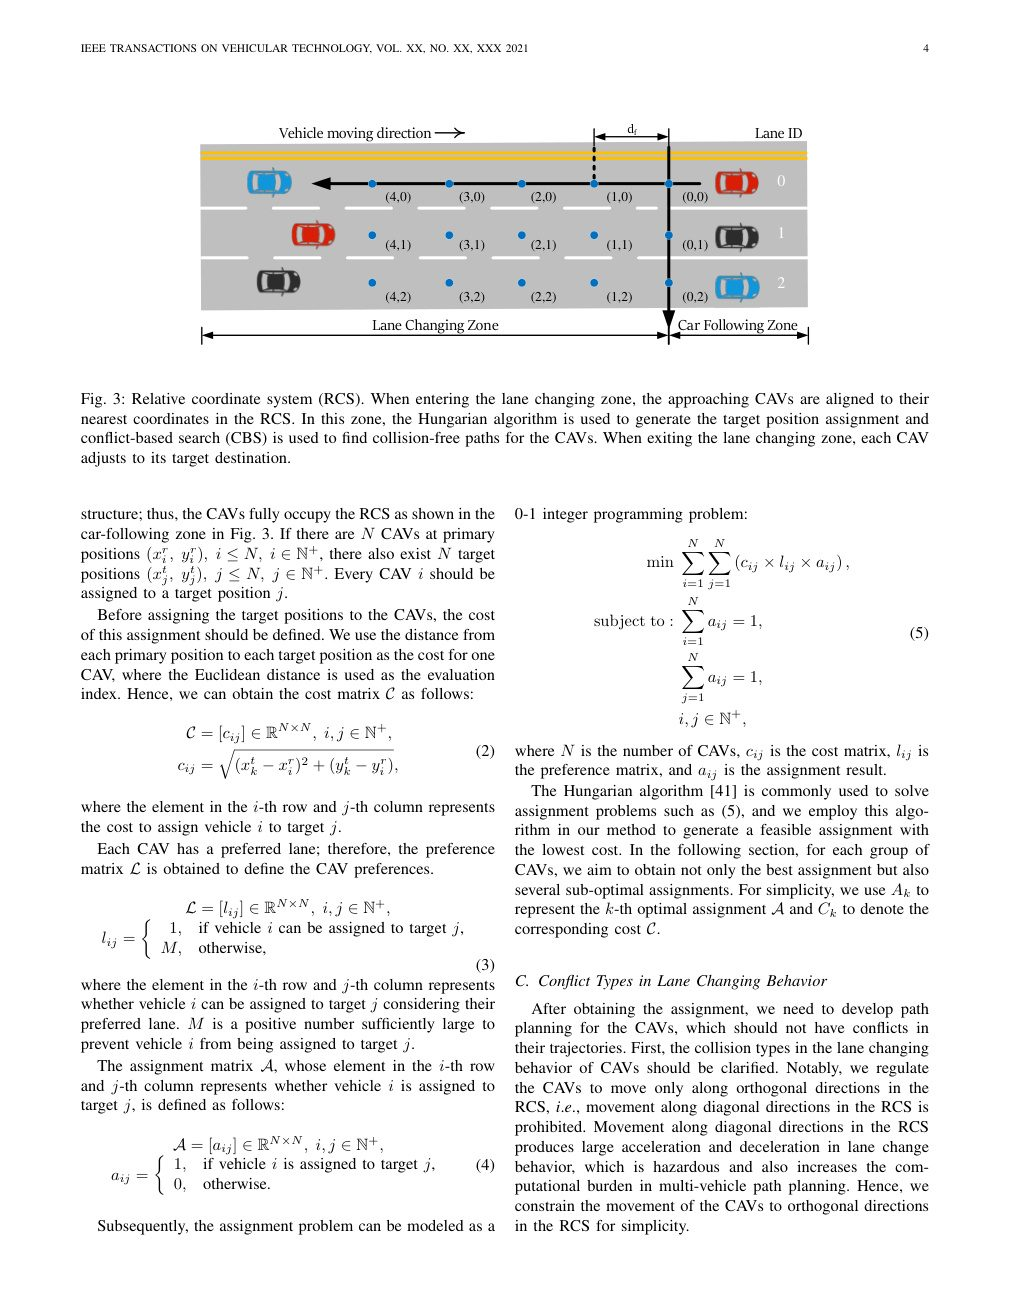
\includegraphics[width=0.92\linewidth]{../../assets/P03_chen2021lanechanging/02_modeling_or_problem_setup_p4.jpg}
\caption{建模或问题设定页 / Modeling or problem-setup page (p.4, full\_page). 这张截图用于把笔记中的抽象概念拉回原论文页面，便于你平行阅读原文、公式、图表和实验设置。 与当前课题的连接：Useful for discussing route-template/lane-choice extensions beyond the current fixed-route JSSP formulation.}
\end{figure}

\begin{figure}[H]
\centering
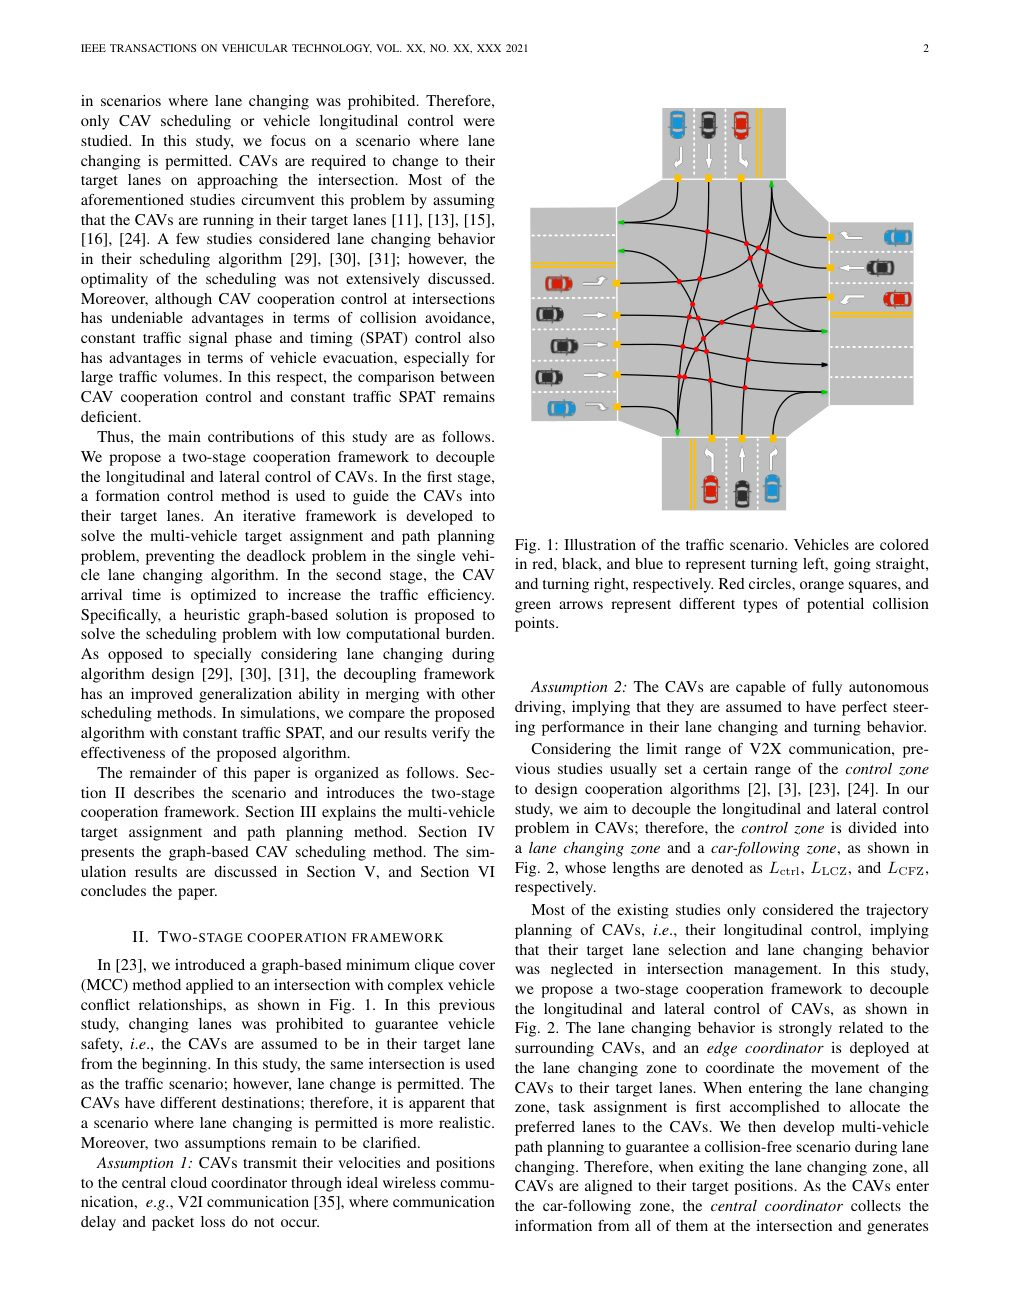
\includegraphics[width=0.92\linewidth]{../../assets/P03_chen2021lanechanging/03_core_method_or_algorithm_p2.jpg}
\caption{核心方法或算法页 / Core method or algorithm page (p.2, full\_page). 这张截图用于把笔记中的抽象概念拉回原论文页面，便于你平行阅读原文、公式、图表和实验设置。 与当前课题的连接：Useful for discussing route-template/lane-choice extensions beyond the current fixed-route JSSP formulation.}
\end{figure}

\begin{figure}[H]
\centering
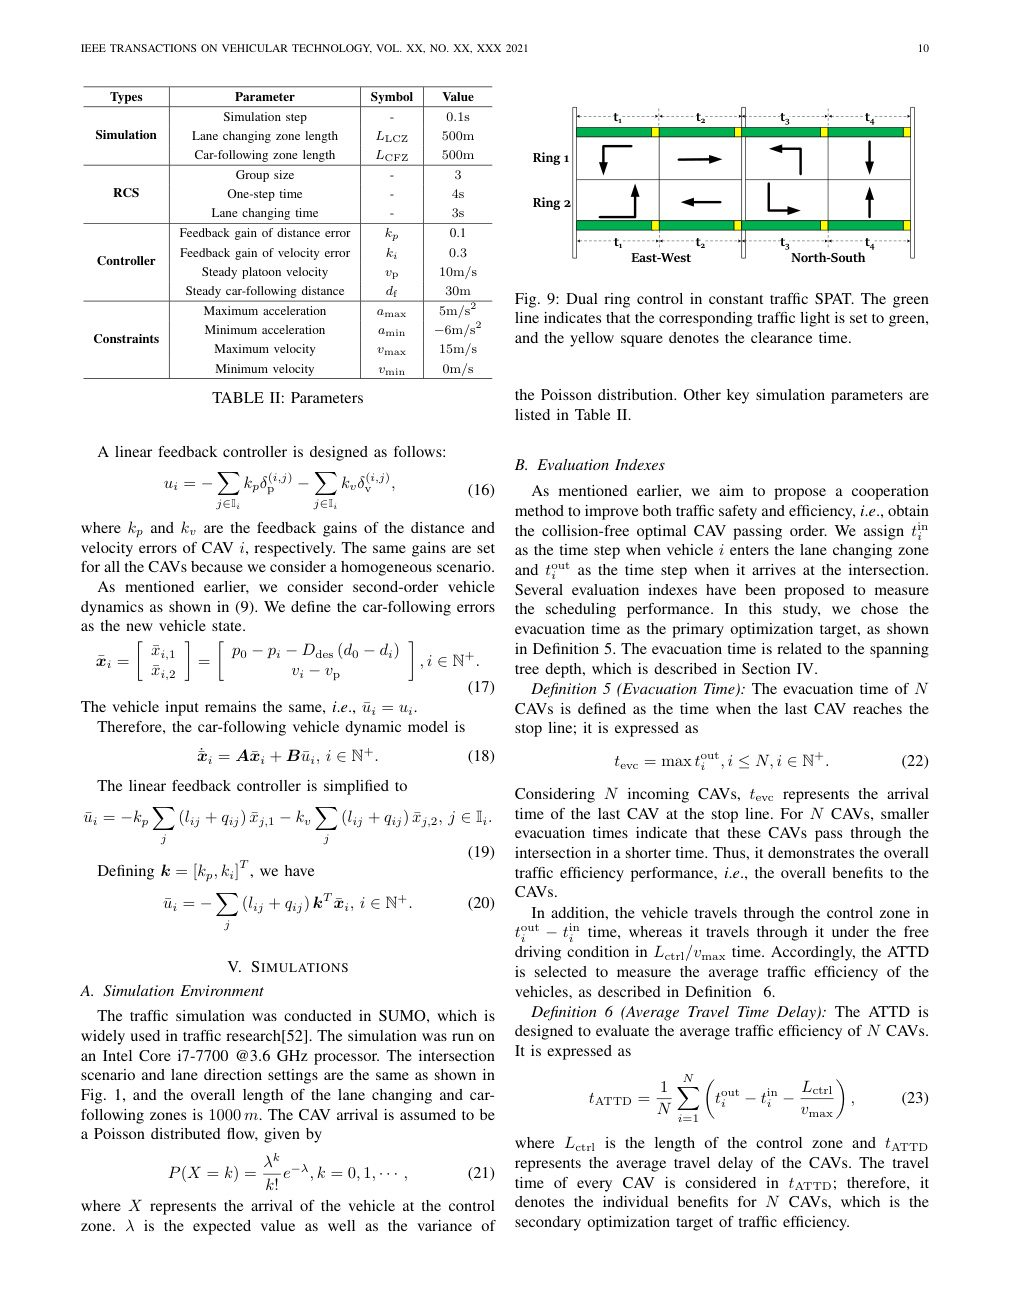
\includegraphics[width=0.92\linewidth]{../../assets/P03_chen2021lanechanging/04_experiments_or_results_p10.jpg}
\caption{实验或结果页 / Experiments or results page (p.10, full\_page). 这张截图用于把笔记中的抽象概念拉回原论文页面，便于你平行阅读原文、公式、图表和实验设置。 与当前课题的连接：Useful for discussing route-template/lane-choice extensions beyond the current fixed-route JSSP formulation.}
\end{figure}

\begin{figure}[H]
\centering
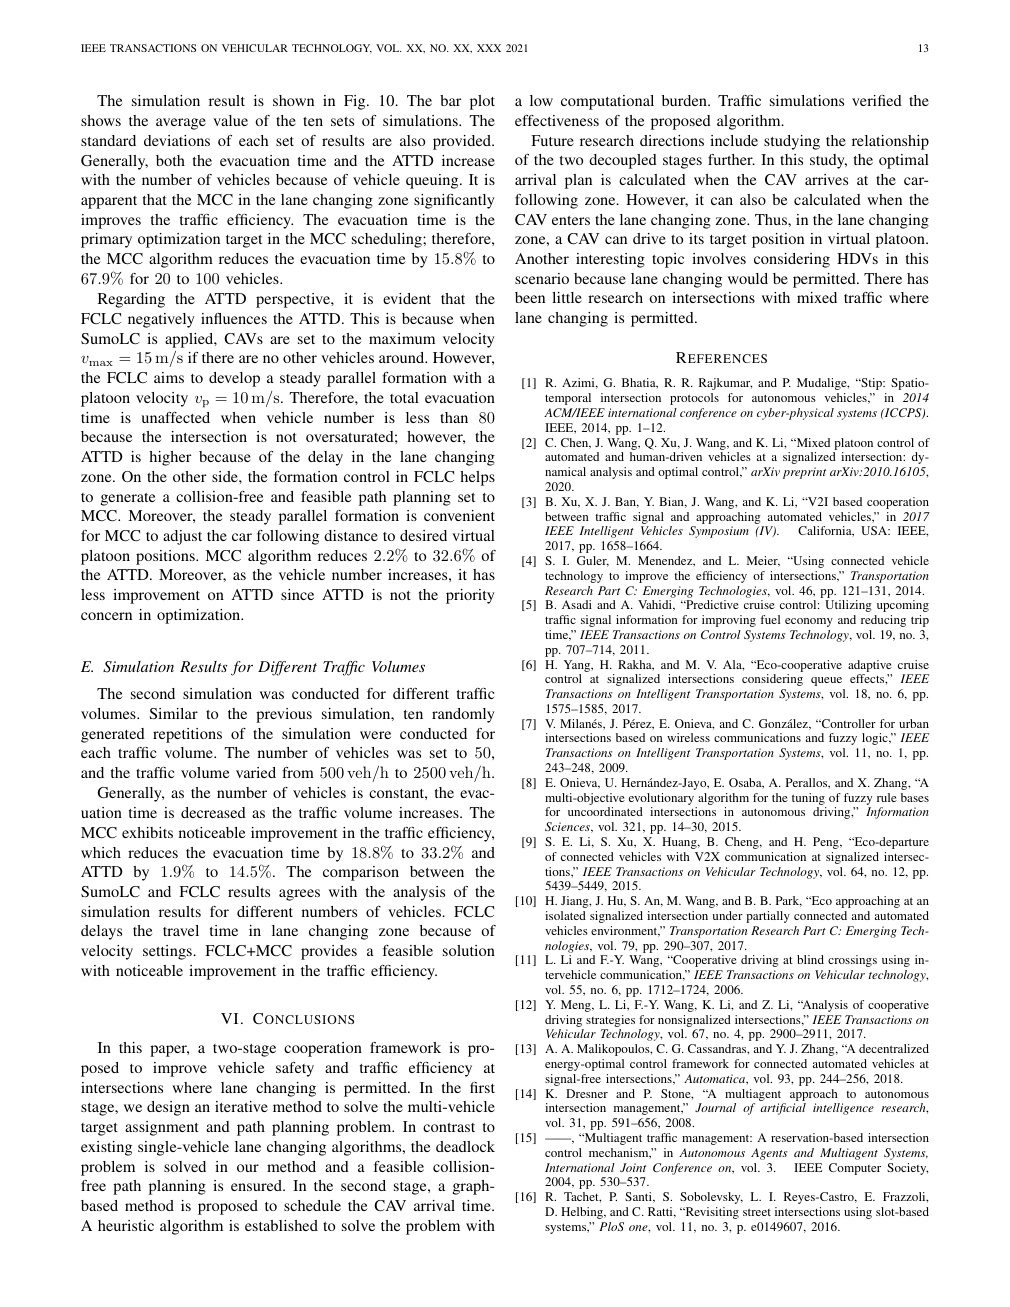
\includegraphics[width=0.92\linewidth]{../../assets/P03_chen2021lanechanging/05_conclusion_or_limitations_p13.jpg}
\caption{结论或局限页 / Conclusion or limitations page (p.13, full\_page). 这张截图用于把笔记中的抽象概念拉回原论文页面，便于你平行阅读原文、公式、图表和实验设置。 与当前课题的连接：Useful for discussing route-template/lane-choice extensions beyond the current fixed-route JSSP formulation.}
\end{figure}


\section{章节精读与逐段导读 / Section-by-Section Deep Reading \& Walkthrough}
\subsection*{p.1 I. INTRODUCTION}
\textbf{章节目标 / Learning goal：} 建立研究动机：为什么传统信号控制、FCFS 或单车控制不足以处理该论文关注的交叉口协同问题。

Understand why the paper needs a new coordination method rather than a standard signal, FCFS, or single-vehicle controller.

\textbf{关键论点 / Key argument：} 这一部分通常把痛点落到 Lane changing + arrival scheduling：既要提高效率，又要保持安全与在线可执行。

\textbf{技术焦点 / Technical focus：} 精读时标出作者批判的 baseline、场景假设、交通参与者类型和隐含优化目标。

\textbf{审稿追问 / Reviewer question：} 作者指出的痛点是否真的需要新方法，还是可以由更强的优化器/更保守规则解决？

\subsection*{p.2 II. T WO-STAGE COOPERATION FRAMEWORK}
\textbf{章节目标 / Learning goal：} 解释算法如何把模型转化为可执行决策，并说明在线运行机制。

Trace how the paper turns the model into executable online decisions.

\textbf{关键论点 / Key argument：} 框架先求多车目标分配与路径规划，再基于最终路径构建冲突图并求到达时间。这样横向变道改变冲突关系，纵向调度再处理被改变后的路口资源竞争。

\textbf{技术焦点 / Technical focus：} 画出输入、核心求解器、输出和安全检查接口，明确哪些步骤是优化、哪些是规则、哪些是学习。

\textbf{审稿追问 / Reviewer question：} 若算法某一步失败，论文有没有 fallback、重规划或安全过滤机制？

\subsection*{p.3 III. M ULTI-VEHICLE TARGET ASSIGNMENT AND PATH}
\textbf{章节目标 / Learning goal：} 承接前后章节，补充局部定义、案例或实现细节。

Recover implementation details needed for reproduction.

\textbf{关键论点 / Key argument：} 这类章节常常不是主贡献，但决定你能否真正复现方法。

\textbf{技术焦点 / Technical focus：} 检查它是否给出了参数、伪代码、场景划分或实现细节。

\textbf{审稿追问 / Reviewer question：} 跳过该节会不会导致公式或实验无法复现？

\subsection*{p.6 1. However, we}
\textbf{章节目标 / Learning goal：} 承接前后章节，补充局部定义、案例或实现细节。

Recover implementation details needed for reproduction.

\textbf{关键论点 / Key argument：} 这类章节常常不是主贡献，但决定你能否真正复现方法。

\textbf{技术焦点 / Technical focus：} 检查它是否给出了参数、伪代码、场景划分或实现细节。

\textbf{审稿追问 / Reviewer question：} 跳过该节会不会导致公式或实验无法复现？

\subsection*{p.7 IV. CAV S CHEDULING AT UNSIGNALIZED INTERSECTIONS}
\textbf{章节目标 / Learning goal：} 承接前后章节，补充局部定义、案例或实现细节。

Recover implementation details needed for reproduction.

\textbf{关键论点 / Key argument：} 这类章节常常不是主贡献，但决定你能否真正复现方法。

\textbf{技术焦点 / Technical focus：} 检查它是否给出了参数、伪代码、场景划分或实现细节。

\textbf{审稿追问 / Reviewer question：} 跳过该节会不会导致公式或实验无法复现？

\subsection*{p.9 4. This also indicates that the theoretical evacuation times}
\textbf{章节目标 / Learning goal：} 承接前后章节，补充局部定义、案例或实现细节。

Recover implementation details needed for reproduction.

\textbf{关键论点 / Key argument：} 这类章节常常不是主贡献，但决定你能否真正复现方法。

\textbf{技术焦点 / Technical focus：} 检查它是否给出了参数、伪代码、场景划分或实现细节。

\textbf{审稿追问 / Reviewer question：} 跳过该节会不会导致公式或实验无法复现？

\subsection*{p.9 6. We have proved that this can be solved by exchanging the}
\textbf{章节目标 / Learning goal：} 承接前后章节，补充局部定义、案例或实现细节。

Recover implementation details needed for reproduction.

\textbf{关键论点 / Key argument：} 这类章节常常不是主贡献，但决定你能否真正复现方法。

\textbf{技术焦点 / Technical focus：} 检查它是否给出了参数、伪代码、场景划分或实现细节。

\textbf{审稿追问 / Reviewer question：} 跳过该节会不会导致公式或实验无法复现？

\subsection*{p.10 V. SIMULATIONS}
\textbf{章节目标 / Learning goal：} 验证方法是否在公平基准下改善效率、安全、能耗或计算时间。

Check whether the claimed improvements are supported by fair baselines and meaningful metrics.

\textbf{关键论点 / Key argument：} 实验应与论文声称的贡献闭环：Numerical simulations for different vehicle counts and traffic volumes.

\textbf{技术焦点 / Technical focus：} 重点追踪指标：平均延误、总行程时间、完成变道比例、冲突避免成功率和交通量敏感性。 同时检查仿真平台、交通需求和随机性设置。

\textbf{审稿追问 / Reviewer question：} 实验是否只展示平均收益，还是覆盖了高密度、异常扰动和失败案例？


\subsection{逐段式导读 / Paragraph-Level Walkthrough}
\paragraph{Opening motivation / 开篇动机段}先把作者的痛点翻译成一句博士问题：当车辆可以变道或选择目标车道时，如何联合决定路径/车道与无冲突到达时间？ 读这一段时不要急着接受动机，要追问传统 FCFS、信号灯或保守 MPC 为什么不足。

Turn the opening motivation into one doctoral-level question and test whether the paper truly needs a new method.

\paragraph{Assumption and setting / 假设与场景段}把车辆类型、通信条件、路口类型和动力学假设列成表。该文的关键边界包括：车辆可执行规划出的变道动作，周围交通允许形成编队。；车道级地图和目标车道需求已知。；变道安全约束可以被简化成可规划的路径/队形约束。

List vehicle type, communication, intersection setting, and dynamics assumptions before reading the equations.

\paragraph{Model and notation / 模型与符号段}围绕核心公式“联合车道分配与到达时间优化 / Joint lane assignment and arrival scheduling”复写符号表，确认每个变量是决策变量、状态变量、参数还是约束阈值。

Rewrite the symbol table around the core formulation and classify variables as states, decisions, parameters, or constraints.

\paragraph{Algorithm mechanism / 算法机制段}把算法读成一条数据流：输入交通状态，执行 Two-stage framework decoupling lateral lane assignment/path planning from graph-based arrival scheduling with minimum clique cover.，输出可执行通行/控制决策，并检查安全接口。

Read the algorithm as a dataflow from traffic state to executable sequence/control decision, with explicit safety interfaces.

\paragraph{Experiment and evidence / 实验证据段}不要只看作者报告的提升，要检查基准、公平性和指标。本文验证描述为：Numerical simulations for different vehicle counts and traffic volumes.

Go beyond reported gains and inspect baselines, fairness, metrics, and computation time.

\paragraph{Reviewer synthesis / 审稿式总结段}最后把贡献拆成可发表与需补强两部分。对你课题最直接的用途是：Useful for discussing route-template/lane-choice extensions beyond the current fixed-route JSSP formulation.

Separate publishable contribution from missing evidence, then connect the result to your own thesis architecture.


\section{技术路线图与贡献量评估 / Technical Route \& Contribution Matrix}
\begin{longtable}{p{0.08\linewidth}p{0.24\linewidth}p{0.58\linewidth}}
\toprule
Step & Stage / 阶段 & Content / 内容\\
\midrule
1 & 输入 / Input & 车辆状态、路径/车道、交通需求、信号或协同信息。 \\
2 & 建模 / Modeling & 联合车道分配与到达时间优化 / Joint lane assignment and arrival scheduling \\
3 & 核心求解 / Core solver & Two-stage framework decoupling lateral lane assignment/path planning from graph-based arrival scheduling with minimum clique cover. \\
4 & 安全接口 / Safety interface & Conflict-free arrival scheduling and formation-control assumptions prevent incompatible movements. \\
5 & 平滑与效率 / Smoothing and efficiency & Improves traffic efficiency by choosing target lanes and arrival schedules that avoid unnecessary queuing. \\
6 & 验证 / Validation & Numerical simulations for different vehicle counts and traffic volumes. \\
\bottomrule
\end{longtable}

\begin{longtable}{p{0.34\linewidth}p{0.14\linewidth}p{0.42\linewidth}}
\toprule
Dimension / 维度 & Score & Comment / 评语\\
\midrule
理论贡献 / Theoretical contribution & 3/5 & 联合车道分配与到达时间优化 / Joint lane assignment and arrival scheduling \\
算法贡献 / Algorithmic contribution & 4/5 & Two-stage framework decoupling lateral lane assignment/path planning from graph-based arrival scheduling with minimum clique cover. \\
实验贡献 / Experimental contribution & 3/5 & Numerical simulations for different vehicle counts and traffic volumes. \\
工程贡献 / Engineering contribution & 3/5 & Conflict-free arrival scheduling and formation-control assumptions prevent incompatible movements. \\
博士课题价值 / PhD relevance & 4/5 & Useful for discussing route-template/lane-choice extensions beyond the current fixed-route JSSP formulation. \\
\bottomrule
\end{longtable}

\section{理论方法论深度解构 / Methodology \& Theoretical Framework}
\subsection{问题数学建模 / Mathematical Formulation}
\textbf{联合车道分配与到达时间优化 / Joint lane assignment and arrival scheduling}
\[
\min_{l_i,t_i}\; \sum_{i\in V}\left(\alpha\,d_i(l_i)+\beta\,|t_i-t_i^{des}|\right)\quad \text{s.t.}\; (i,j)\in E(l)\Rightarrow |t_i-t_j|\ge \tau_{ij}
\]
\begin{longtable}{p{0.16\linewidth}p{0.25\linewidth}p{0.25\linewidth}p{0.25\linewidth}}
\toprule
Symbol / 符号 & 含义 & Meaning & Role / 建模作用\\
\midrule
l\_i & 目标车道 & target lane & 横向规划决策变量 \\
t\_i & 车辆到达冲突区时间 & arrival time at conflict zone & 纵向调度决策变量 \\
d\_i(l\_i) & 变道代价 & lane-changing cost & 衡量横向操作复杂度 \\
E(l) & 由车道选择诱导的冲突边集 & lane-induced conflict edges & 说明横向选择会改变调度约束 \\
tau\_ij & 安全时间间隔 & safety headway & 保证冲突车辆时间分离 \\
\bottomrule
\end{longtable}

\subsection{核心算法架构 / Core Algorithm Layout}
框架先求多车目标分配与路径规划，再基于最终路径构建冲突图并求到达时间。这样横向变道改变冲突关系，纵向调度再处理被改变后的路口资源竞争。

The framework first assigns target lanes/paths, then constructs a conflict graph for those paths and computes a conflict-free arrival schedule.

\subsection{收敛性、稳定性或实时性 / Convergence, Stability, Real-Time Feasibility}
分阶段设计提高实时性，但牺牲联合最优性；如果第一阶段车道选择失误，第二阶段只能在较差冲突结构上补救。

The two-stage decomposition is tractable but not globally optimal; poor lane assignment can constrain the downstream scheduler.

\subsection{潜在假设与边界条件 / Assumptions \& Boundary Conditions}
\begin{itemize}
\item 车辆可执行规划出的变道动作，周围交通允许形成编队。
\item 车道级地图和目标车道需求已知。
\item 变道安全约束可以被简化成可规划的路径/队形约束。
\end{itemize}


\section{实验验证与结果评判 / Experimental Validation \& Result Evaluation}
\textbf{Baselines \& Environment / 基准与环境：} 固定车道策略、无变道调度、FCFS 和基于图的到达调度。

\textbf{Validation / 验证：} Numerical simulations for different vehicle counts and traffic volumes.

\textbf{Metrics / 指标：} 平均延误、总行程时间、完成变道比例、冲突避免成功率和交通量敏感性。

\textbf{Ablation / 消融：} 最关键消融是去掉 lane-changing stage，对比是否真的改善调度；还应测试高密度下变道失败的退化策略。

\textbf{Reviewer reading / 审稿式阅读提醒：} 阅读实验时不要只看平均值；应检查交通密度、车流方向、随机种子、失败案例和计算耗时。For doctoral reading, inspect density regimes, demand patterns, random seeds, failure cases, and computation time rather than only mean improvements.

\subsection{图表阅读线索 / Figure and Table Reading Cues}
PDF extraction detected approximately 44 figure references and 6 table references. Exact captions remain in the original PDF; the bilingual cues below tell you what to inspect first.

\begin{longtable}{p{0.24\linewidth}p{0.30\linewidth}p{0.36\linewidth}}
\toprule
图表名称 & Figure/Table Name & Reading focus / 阅读重点\\
\midrule
系统框架图 & system framework diagram & 先确认输入、决策层、控制层和安全约束之间的数据流。 \\
冲突关系图 / 通行顺序图 & conflict-relation or passing-order graph & 把节点、边类型和先后约束翻译成 JSSP 的作业、机器和析取约束。 \\
实验指标对比图表 & experimental metric comparison plots/tables & 重点看平均值之外的密度变化、失败场景、计算时间和方差。 \\
\bottomrule
\end{longtable}

\section{审稿人视角：批判性思考与未来方向 / Critical Thinking \& Future Directions}
\subsection{论文局限性 / Limitations \& Weaknesses}
\begin{itemize}
\item 文本与同作者早期图调度工作高度相关，独立贡献需谨慎引用。
\item 横向控制细节和人类驾驶干扰不足。
\item 两阶段解耦可能错过更优的路径-时间联合解。
\end{itemize}


\subsection{博士课题拓展点 / Research Extensions for PhD}
\begin{itemize}
\item 用双层优化 (bi-level optimization) 同时学习车道选择和 JSSP 排序。
\item 为变道失败设计可恢复调度 (recoverable scheduling)，让路口管理器在线回滚目标车道。
\item 把车道选择看成 route-template selection，扩展当前固定路线假设。
\end{itemize}


\subsection{如何服务当前课题 / Use in This Project}
Useful for discussing route-template/lane-choice extensions beyond the current fixed-route JSSP formulation.

\section{交互式可视化与 PDF 排版蓝图 / Interactive Visualization \& PDF Layout Blueprint}
\textbf{动态参数 / Parameter：} 可变道车辆比例 / Lane-change-enabled ratio, range [0, 1] .

比例增加会提高调度自由度，但过高时变道冲突和局部扰动也会增加。

More lane-change freedom improves scheduling flexibility but can add lateral conflicts.

\subsection{HTML 结构化布局建议 / HTML Structuring}
\begin{itemize}
\item 顶部固定 metadata bar：题名、作者、年份、主题、PDF 页数。
\item 左侧目录/section navigator，右侧为五大精读模块。
\item 公式卡片使用 <pre> 或 LaTeX block，紧跟符号表。
\item 审稿人批注用 reviewer-note block，博士拓展用 research-idea list。
\item 交互参数用 input[type=range] + canvas 曲线，打印 PDF 时隐藏交互控件但保留解释。
\end{itemize}


\section{来源锚点与逐节阅读路径 / Source Anchors \& Section-by-Section Reading Map}
\begin{longtable}{p{0.14\linewidth}p{0.76\linewidth}}
\toprule
Page & Extracted heading\\
\midrule
p.1 & I. INTRODUCTION \\
p.2 & II. T WO-STAGE COOPERATION FRAMEWORK \\
p.10 & V. SIMULATIONS \\
\bottomrule
\end{longtable}

\paragraph{p.1 I. INTRODUCTION}定位问题背景、研究缺口和为什么现有保守/非协同方法不足。 / Frames the motivation, research gap, and limits of conservative or non-cooperative methods.

\paragraph{p.2 II. T WO-STAGE COOPERATION FRAMEWORK}给出算法流程和求解机制，应重点追踪输入、输出和安全接口。 / Gives the algorithmic mechanism; track inputs, outputs, and safety interfaces.

\paragraph{p.3 III. M ULTI-VEHICLE TARGET ASSIGNMENT AND PATH}作为局部论证段落阅读，关注它如何服务主问题。 / Read as a local argument and ask how it supports the main question.

\paragraph{p.6 1. However, we}作为局部论证段落阅读，关注它如何服务主问题。 / Read as a local argument and ask how it supports the main question.

\paragraph{p.7 IV. CAV S CHEDULING AT UNSIGNALIZED INTERSECTIONS}作为局部论证段落阅读，关注它如何服务主问题。 / Read as a local argument and ask how it supports the main question.

\paragraph{p.9 4. This also indicates that the theoretical evacuation times}作为局部论证段落阅读，关注它如何服务主问题。 / Read as a local argument and ask how it supports the main question.

\paragraph{p.9 6. We have proved that this can be solved by exchanging the}作为局部论证段落阅读，关注它如何服务主问题。 / Read as a local argument and ask how it supports the main question.

\paragraph{p.10 V. SIMULATIONS}检验方法是否真的改善效率、安全或能耗；要关注基准是否公平。 / Tests efficiency, safety, or energy claims; inspect whether baselines are fair.


\end{document}
